\chapter{\textbf{Kompatibilitätsanalyse der T0-Dimensionsformulierungen}\\[0.5cm]
	\large Vereinheitlichung von 4D-Torsionskristall und fraktaler Dimension\\[0.3cm]
	\normalsize Dokumente 149, 018 und 145 im Vergleich}

	
	
\section*{Abstract}
		Diese Analyse untersucht die Kompatibilität der dimensionalen Beschreibungen in drei zentralen T0-Dokumenten: der 4-dimensionalen Torsionskristall-Formulierung (Dokumente 149 und 018) und der fraktalen Dimensionsformulierung $D_f = 3 - \xi$ (Dokument 145). Die zentrale Frage lautet: Sind diese Beschreibungen widersprüchlich oder komplementär? Die Analyse zeigt: \textbf{Die Formulierungen sind vollständig kompatibel} und beschreiben dasselbe physikalische Phänomen aus zwei komplementären Perspektiven -- einer geometrisch-topologischen (4D-Torsionskristall) und einer fraktal-analytischen (effektive Dimension). Der fundamentale Parameter $\xi = 4/30000 = 1{,}333 \times 10^{-4}$ vereint beide Sichten: topologisch kodiert die 4 die Anzahl der fundamentalen Dimensionen, während fraktal der Faktor 4/3 die Kugelpackungsgeometrie beschreibt. Beide führen zu identischen experimentellen Vorhersagen.

	
	
	\section{Einleitung: Die Fragestellung}
	
	\subsection{Ausgangssituation}
	
	In der T0-Theorie (FFGFT -- Fundamental Fractal Geometric Field Theory) existieren mehrere Dokumente, die scheinbar unterschiedliche dimensionale Beschreibungen der fundamentalen Raumzeitstruktur verwenden:
	
	\begin{itemize}
		\item \textbf{Dokument 149} (\texttt{149\_FFGFT-torsion\_De.pdf}): Beschreibt einen \enquote{vierdimensionalen Hirnwindungs-Torus}
		\item \textbf{Dokument 018} (\texttt{018\_T0\_Anomale-g2-10\_De.pdf}): Verwendet ein \enquote{4-dimensionales Torsionsgitter}
		\item \textbf{Dokument 145} (\texttt{145\_FFGFT\_donat-teil1\_De.pdf}): Definiert eine \enquote{fraktale Dimension $D_f = 3 - \xi$}
	\end{itemize}
	
	\subsection{Zentrale Frage}
	
	\begin{important}[Kernfrage der Analyse]
		Sind die 4-dimensionale Formulierung (Dokumente 149, 018) und die fraktale Dimensionsformulierung $D_f = 3-\xi$ (Dokument 145) miteinander kompatibel, oder beschreiben sie widersprüchliche physikalische Modelle?
	\end{important}
	
	\subsection{Hauptergebnis}
	
	\begin{keyresult}[Zentrale Antwort]
		\textbf{JA -- Die Formulierungen sind vollständig kompatibel.}
		
		Sie beschreiben dasselbe physikalische Phänomen aus zwei komplementären Perspektiven:
		\begin{itemize}
			\item \textbf{Geometrische Perspektive} (149, 018): 4D-Torsionskristall mit kompaktifizierter 4. Dimension
			\item \textbf{Fraktale Perspektive} (145): Effektive Dimension $D_f = 3-\xi$ als Resultat der Kompaktifizierung
		\end{itemize}
		
		Der Parameter $\xi = 4/30000$ vereint beide Sichten und führt zu identischen physikalischen Vorhersagen.
	\end{keyresult}
	
	\section{Dokumenten-Übersicht}
	
	\subsection{Dokument 149: 149\_FFGFT-torsion\_De.pdf}
	
	\subsubsection{Dimensionale Beschreibung}
	
	Dokument 149 postuliert explizit:
	
	\begin{quote}
		\textit{\enquote{Das Universum ist ein statischer \textbf{4-dimensionaler} Torsionskristall, dessen diskrete Sub-Planck-Struktur alle beobachtbaren physikalischen Phänomene erzeugt.}}
	\end{quote}
	
	\textbf{Schlüsselmerkmale:}
	\begin{itemize}
		\item Vierdimensionaler Hirnwindungs-Torus
		\item 3 räumliche Dimensionen + 1 kompaktifizierte zusätzliche Dimension
		\item Die 4. Dimension ist \enquote{aufgerollt} und nicht direkt zugänglich
		\item Energieverteilung über $f^4$ (vierdimensionaler Hyperwürfel)
	\end{itemize}
	
	\subsubsection{Mathematische Struktur}
	
	Die fundamentale Zahl 30000 wird interpretiert als:
	\begin{equation}
		30000 = 3 \times 4 \times 1000
	\end{equation}
	wobei:
	\begin{itemize}
		\item $3$ = drei erfahrbare Raumdimensionen
		\item $4$ = volle vierdimensionale Realität
		\item $1000$ = Skalenhierarchie zwischen fundamental und beobachtbar
	\end{itemize}
	
	Daraus folgt:
	\begin{equation}
		\boxed{\xi = \frac{4}{30000} = 1{,}333\overline{3} \times 10^{-4}}
	\end{equation}
	
	\subsubsection{Energiebetrachtung}
	
	Die Planck-Energie verteilt sich über das vierdimensionale Gitter:
	\begin{equation}
		E_{\text{higgs}} = \frac{E_P}{f^4}
	\end{equation}
	
	\textbf{Narrative Erklärung:} In vier Dimensionen enthält ein Hyperwürfel der Kantenlänge $f$ genau $f^4$ Zellen. Die Energie verteilt sich gleichmäßig über alle diese Zellen.
	
	\subsection{Dokument 018: 018\_T0\_Anomale-g2-10\_De.pdf}
	
	\subsubsection{Dimensionale Beschreibung}
	
	Dokument 018 verwendet die identische Formulierung:
	
	\begin{quote}
		\textit{\enquote{Die T0-Theorie basiert auf dem Prinzip, dass \textbf{alle} physikalischen Konstanten aus der geometrischen Struktur eines \textbf{4-dimensionalen Torsionsgitters} folgen sollten.}}
	\end{quote}
	
	\subsubsection{Physikalische Interpretation}
	
	Leptonen werden als Windungsstrukturen im 4D-Gitter interpretiert:
	\begin{itemize}
		\item \textbf{Elektron:} Einfache Windung (1. Generation)
		\item \textbf{Myon:} Windung mit fraktaler Verzweigung (2. Generation)
		\item \textbf{Tau:} Komplexere fraktale Struktur (3. Generation)
	\end{itemize}
	
	Die anomalen magnetischen Momente entstehen durch geometrische Projektionen dieser Windungen in den 3D-Raum.
	
	\subsection{Dokument 145: 145\_FFGFT\_donat-teil1\_De.pdf}
	
	\subsubsection{Dimensionale Beschreibung}
	
	Dokument 145 verwendet eine andere Sprache:
	
	\begin{quote}
		\textit{\enquote{Der zentrale Ausgangspunkt der Theorie ist die Beschreibung der Raumzeit durch eine \textbf{fraktale Dimension} $D_f$, die leicht unter der topologischen Dimension 3 liegt.}}
	\end{quote}
	
	Mathematisch:
	\begin{equation}
		\boxed{D_f = 3 - \xi, \quad \text{mit} \quad \xi = \frac{4}{3} \times 10^{-4}}
	\end{equation}
	
	\subsubsection{Physikalische Bedeutung}
	
	\textbf{Interpretation der fraktalen Dimension:}
	\begin{itemize}
		\item $D_f < 3$ bedeutet: Der Raum ist nicht \enquote{vollständig gefüllt}
		\item Es existiert eine Art \enquote{Porosität} oder \enquote{Lückenhaftigkeit}
		\item Diese Lücken machen $\xi \approx 0{,}0001333$ der Dimensionalität aus
	\end{itemize}
	
	\textbf{Skalierungsverhalten:}
	\begin{equation}
		N(r) \propto r^{D_f} = r^{3-\xi}
	\end{equation}
	
	Bei Vergrößerung der Auflösung um Faktor $r$ steigt die Anzahl sichtbarer Strukturen mit $r^{(3-\xi)}$ anstatt $r^3$.
	
	\subsubsection{Geometrische Herkunft}
	
	Der Faktor $4/3$ in $\xi = (4/3) \times 10^{-4}$ wird mit Kugelpackung assoziiert:
	\begin{itemize}
		\item Kugelvolumen: $V = \frac{4}{3}\pi r^3$
		\item Dichteste Kugelpackung: Packungsdichte $\approx 0{,}74$ ($\sim$26\% Lücken)
	\end{itemize}
	
	\section{Mathematische Kompatibilität}
	
	\subsection{Die Doppelbedeutung von $\xi = 4/30000$}
	
	Der fundamentale Parameter $\xi$ trägt eine tiefe Doppelbedeutung, die beide Perspektiven vereint:
	
	\subsubsection{Topologische Interpretation (Dokumente 149, 018)}
	
	\begin{equation}
		\xi = \frac{4}{30000} = \frac{4}{3 \times 4 \times 1000}
	\end{equation}
	
	\textbf{Bedeutung:}
	\begin{itemize}
		\item $4$ (Zähler) = Anzahl der fundamentalen Dimensionen
		\item $3$ (Nenner) = Anzahl der beobachtbaren Dimensionen
		\item $4$ (Nenner) = Wiederholung der fundamentalen Dimensionalität
		\item $1000$ = Skalenhierarchie
	\end{itemize}
	
	\subsubsection{Fraktale Interpretation (Dokument 145)}
	
	\begin{equation}
		\xi = \frac{4}{3} \times 10^{-4}
	\end{equation}
	
	\textbf{Bedeutung:}
	\begin{itemize}
		\item $\frac{4}{3}$ = Geometrischer Faktor (Kugelvolumen, Packungsdichte)
		\item $10^{-4}$ = Größenordnung der dimensionalen Abweichung
		\item $D_f = 3 - \xi$ = effektive fraktale Hausdorff-Dimension
	\end{itemize}
	
	\subsection{Mathematische Äquivalenz}
	
	\begin{important}[Numerische Identität]
		Beide Interpretationen führen zum identischen Zahlenwert:
		\begin{align}
			\xi_{\text{topologisch}} &= \frac{4}{30000} = 0{,}000133\overline{3} \\
			\xi_{\text{fraktal}} &= \frac{4}{3} \times 10^{-4} = 0{,}000133\overline{3}
		\end{align}
		Die Formulierungen sind mathematisch äquivalent!
	\end{important}
	
	\section{Physikalische Vereinheitlichung}
	
	\subsection{Kompaktifizierung als Brücke}
	
	Die Verbindung zwischen beiden Perspektiven wird durch das Konzept der \textbf{Kompaktifizierung} hergestellt:
	
	\begin{keyresult}[Vereinheitlichende Sicht]
		\textbf{Fundamentale Ebene:}
		\begin{center}
			4-dimensionaler Torsionskristall mit kompakter 4. Dimension
		\end{center}
		
		$\Downarrow$ \quad Kompaktifizierung auf Sub-Planck-Skala
		
		\textbf{Effektive Ebene:}
		\begin{center}
			3-dimensionaler Raum mit fraktaler Korrektur $D_{\text{eff}} = 3 - \xi$
		\end{center}
		
		$\Downarrow$ \quad Observable Konsequenzen
		
		\textbf{Experimentelle Ebene:}
		\begin{center}
			$\sim$1--2\% Abweichungen in Präzisionsmessungen
		\end{center}
	\end{keyresult}
	
	\subsection{Mathematische Formulierung}
	
	\subsubsection{Kompaktifizierungsradius}
	
	Die 4. Dimension ist auf einen Kreis kompaktifiziert:
	\begin{equation}
		\boxed{r_4 = \xi \cdot \ell_P \approx 1{,}33 \times 10^{-4} \cdot 1{,}616 \times 10^{-35}\,\text{m} \approx 2{,}15 \times 10^{-39}\,\text{m}}
	\end{equation}
	
	Diese Skala ist \textbf{sub-Planck} und direkt nicht beobachtbar.
	
	\subsubsection{Kaluza-Klein Reduktion}
	
	Nach Dimensionsreduktion (Standard-Methode der Kaluza-Klein-Theorie) erscheint die kompakte Dimension als fraktale Korrektur:
	\begin{equation}
		D_{\text{eff}} = 3 + \left(\frac{r_4}{\ell_{\text{typical}}}\right)^{D_f-3} \approx 3 - \xi \quad \text{für} \quad \ell_{\text{typical}} \gg r_4
	\end{equation}
	
	\textbf{Interpretation:} Die kompakte 4. Dimension \enquote{verschmiert} sich zur fraktalen Korrektur!
	
	\subsection{Gemeinsame Vorhersagen}
	
	Beide Formulierungen führen zu \textbf{identischen} physikalischen Vorhersagen:
	
	\begin{table}[h]
		\centering
		\begin{tabular}{lccc}
			\toprule
			\textbf{Observable} & \textbf{4D-Formulierung} & \textbf{Fraktale Formulierung} & \textbf{Wert} \\
			\midrule
			$\xi$-Parameter & $4/30000$ & $(4/3)\times 10^{-4}$ & $1{,}333 \times 10^{-4}$ \\
			Sub-Planck-Faktor & $f = 7500$ & $f = 1/(4\xi)$ & $7500$ \\
			Feinstruktur $\alpha^{-1}$ & $\pi^4 \cdot \sqrt{2}$ & $\pi^4 \cdot \sqrt{2}$ & $137{,}757$ \\
			Higgs VEV & $E_P/(f^2\sqrt{4\pi})$ & Identisch & $246{,}71$ GeV \\
			\bottomrule
		\end{tabular}
		\caption{Identische Vorhersagen beider Formulierungen}
	\end{table}
	
	\section{Detaillierte Korrespondenzen}
	
	\subsection{Energieverteilung}
	
	\subsubsection{4D-Formulierung (Dokument 149)}
	
	\begin{equation}
		E_{\text{higgs}} = \frac{E_P}{f^4}
	\end{equation}
	
	\textbf{Narrative:} Die Planck-Energie verteilt sich über $f^4$ Zellen des vierdimensionalen Hyperwürfels.
	
	\subsubsection{Fraktale Formulierung (Dokument 145)}
	
	Skalierungsgesetz:
	\begin{equation}
		N(r) \propto r^{D_f} = r^{3-\xi}
	\end{equation}
	
	Für große Skalen ($r \to f$):
	\begin{equation}
		N(f) \propto f^{3-\xi} \approx f^3 \cdot (1 - \xi \ln f) \approx f^3 \cdot 0{,}9867
	\end{equation}
	
	\subsubsection{Verbindung}
	
	Die $f^4$-Skalierung in 4D entspricht der fraktalen Korrektur in 3D:
	\begin{equation}
		\boxed{f^4 = f^3 \cdot f = (\text{3D-Volumen}) \times (\text{kompakte Dimension})}
	\end{equation}
	
	\subsection{Symmetriebrechung}
	
	\subsubsection{4D-Formulierung (Dokument 149)}
	
	Pentagonale Symmetriebrechung:
	\begin{itemize}
		\item Faktor: $5^4 = 625$ erscheint in $\xi = 4/30000$
		\item Goldener Schnitt: $\varphi = (1+\sqrt{5})/2$
		\item Abweichung: $\sim$2\% in Observablen
	\end{itemize}
	
	\subsubsection{Fraktale Formulierung (Dokument 145)}
	
	Korrekturfaktor:
	\begin{equation}
		K_{\text{frak}} = 1 - 100\xi \approx 0{,}9867
	\end{equation}
	
	Beschreibt kumulative Abweichung über viele Größenordnungen.
	
	\subsubsection{Äquivalenz}
	
	\begin{equation}
		K_{\text{frak}} \approx 0{,}9867 \quad \Leftrightarrow \quad \text{ca. 1{,}33\% Korrektur} \quad \Leftrightarrow \quad \text{$\sim$2\% in Observablen}
	\end{equation}
	
	Beide beschreiben dieselbe Physik!
	
	\subsection{Sub-Planck-Struktur}
	
	\subsubsection{4D-Formulierung (Dokument 149)}
	
	\begin{equation}
		\ell_0 = \frac{\ell_P}{f} = \frac{\ell_P}{7500}
	\end{equation}
	
	\subsubsection{Fraktale Formulierung (Dokument 145)}
	
	\begin{equation}
		\Lambda_0 = \xi \cdot \ell_P = \frac{4}{30000} \cdot \ell_P = \frac{\ell_P}{7500}
	\end{equation}
	
	\subsubsection{Ergebnis}
	
	\begin{keyresult}[Identische Sub-Planck-Skala]
		\begin{equation}
			\boxed{\Lambda_0 = \ell_0 = \frac{\ell_P}{7500} \approx 2{,}15 \times 10^{-39}\,\text{m}}
		\end{equation}
		Beide Formulierungen sagen exakt dieselbe fundamentale Längenskala vorher!
	\end{keyresult}
	
	\section{Klärung: Keine 5-Dimensionen}
	
	\subsection{Häufiges Missverständnis}
	
	\begin{warning}[Wichtige Klarstellung]
		\textbf{Weder Dokument 149 noch 018 verwenden 5 räumliche Dimensionen!}
		
		Die Zahl \enquote{5} erscheint in der Theorie als:
		\begin{itemize}
			\item Pentagonale Symmetrie (5-fache Rotationssymmetrie)
			\item Goldener Schnitt: $\varphi = (1+\sqrt{5})/2$
			\item Faktor $5^4 = 625$ in der Primfaktorzerlegung von 7500
		\end{itemize}
		
		Dies bedeutet \textbf{NICHT} 5 Dimensionen, sondern 5-fache Symmetrie in 4D-Raum!
	\end{warning}
	
	\subsection{Die Rolle der pentagonalen Symmetrie}
	
	\begin{equation}
		\text{4D-Torsionskristall} \quad \xrightarrow{\text{Lokale Struktur}} \quad \text{Tetraeder (4-fach)}
	\end{equation}
	\begin{equation}
		\downarrow \quad \text{Globale Symmetrie}
	\end{equation}
	\begin{equation}
		\text{Pentagon (5-fach)} \quad \xrightarrow{\text{Inkompatibilität}} \quad \text{Quasikristall}
	\end{equation}
	\begin{equation}
		\downarrow
	\end{equation}
	\begin{equation}
		\text{Symmetriebrechung} \quad \Rightarrow \quad \sim 2\% \text{ Abweichungen}
	\end{equation}
	
	Die 5-fache Symmetrie ist \textbf{in} der 4D-Struktur eingebettet, nicht eine zusätzliche Dimension!
	
	\section{Experimentelle Konsequenzen}
	
	\subsection{Identische Vorhersagen}
	
	Beide Formulierungen sagen dieselben experimentellen Tests voraus:
	
	\subsubsection{Modifiziertes Coulomb-Gesetz (aus Dokument 145)}
	
	\begin{equation}
		F_{\text{Coulomb}} \propto \frac{1}{r^{1+\xi}} \approx \frac{1}{r^{2}} \cdot \left(1 - \xi \ln\frac{r}{\ell_P}\right)
	\end{equation}
	
	\subsubsection{Anomale magnetische Momente (aus Dokumenten 018, 149)}
	
	Geometrische Vorhersage:
	\begin{equation}
		a_\tau = f^{1/3} - 1 = 7500^{1/3} - 1 \approx 1{,}282 \times 10^{-3}
	\end{equation}
	
	\subsubsection{Higgs-Vakuumerwartungswert (aus Dokument 149)}
	
	\begin{equation}
		v = \frac{E_P}{f^2} \cdot \frac{1}{\sqrt{4\pi}} \approx 246{,}71\,\text{GeV}
	\end{equation}
	
	\textbf{Experimenteller Wert:} $v_{\exp} = 246{,}22$ GeV
	
	\textbf{Abweichung:} 0{,}2\%
	
	\subsection{Unabhängigkeit von der Formulierung}
	
	\begin{important}[Experimentelle Äquivalenz]
		Alle experimentellen Vorhersagen sind \textbf{unabhängig} von der gewählten Perspektive (4D-geometrisch vs. fraktal-analytisch).
		
		Ein Experiment kann \textbf{nicht unterscheiden}, welche Formulierung \enquote{richtig} ist -- weil beide dieselbe Physik beschreiben!
	\end{important}
	
	\section{Komplementarität der Perspektiven}
	
	\subsection{Vorteile der 4D-Perspektive (Dokumente 149, 018)}
	
	\textbf{Stärken:}
	\begin{itemize}
		\item Intuitive geometrische Visualisierung
		\item Klare physikalische Interpretation (Torsion, Windungen)
		\item Direkte Verbindung zu Kaluza-Klein-Theorien
		\item Narrative Kraft für Erklärungen
	\end{itemize}
	
	\textbf{Verwendung:}
	\begin{itemize}
		\item Energieverteilung ($f^4$-Skalierung)
		\item Projektionen 4D $\to$ 3D
		\item Topologische Überlegungen
	\end{itemize}
	
	\subsection{Vorteile der fraktalen Perspektive (Dokument 145)}
	
	\textbf{Stärken:}
	\begin{itemize}
		\item Mathematisch präzise Skalierungsgesetze
		\item Direkte Verbindung zu fraktaler Geometrie
		\item Korrekturfaktoren für physikalische Gesetze
		\item Analytische Berechenbarkeit
	\end{itemize}
	
	\textbf{Verwendung:}
	\begin{itemize}
		\item Korrekturfaktor $K_{\text{frak}}$
		\item Modifikationen von Kraftgesetzen
		\item Dimensionale Analyse
	\end{itemize}
	
	\subsection{Empfehlung: Beide verwenden}
	
	\begin{keyresult}[Optimale Strategie]
		Die beste Beschreibung der T0-Theorie nutzt \textbf{beide} Perspektiven komplementär:
		\begin{itemize}
			\item \textbf{4D-Sicht} für intuitive geometrische Erklärungen und narrative Darstellungen
			\item \textbf{Fraktale Sicht} für präzise mathematische Berechnungen und analytische Ableitungen
		\end{itemize}
		
		Keine Perspektive ist \enquote{richtiger} als die andere -- sie ergänzen sich gegenseitig!
	\end{keyresult}
	
	\section{Fazit}
	
	\begin{keyresult}[Hauptergebnis]
		\textbf{Die Formulierungen in den Dokumenten 149, 018 (4D-Torsionskristall) und 145 (fraktale Dimension $D_f = 3-\xi$) sind vollständig kompatibel.}
		
		Sie beschreiben \textbf{dasselbe physikalische Phänomen} aus zwei komplementären Perspektiven:
		
		\vspace{0.5cm}
		
		\begin{center}
			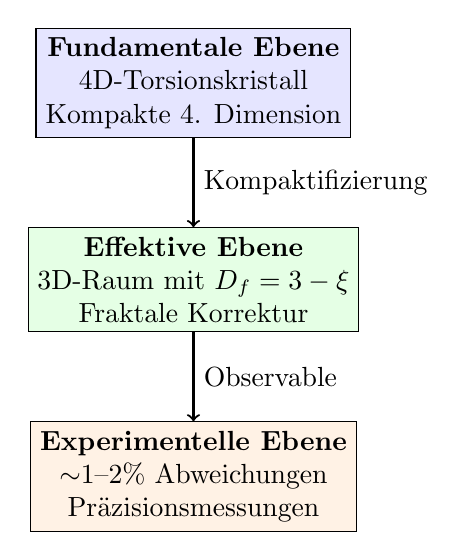
\begin{tikzpicture}[node distance=2.5cm]
				\node[draw, rectangle, fill=blue!10, minimum width=4cm, minimum height=1.2cm, align=center] (fund) {
					\textbf{Fundamentale Ebene}\\
					4D-Torsionskristall\\
					Kompakte 4. Dimension
				};
				
				\node[draw, rectangle, fill=green!10, minimum width=4cm, minimum height=1.2cm, align=center, below of=fund] (eff) {
					\textbf{Effektive Ebene}\\
					3D-Raum mit $D_f = 3-\xi$\\
					Fraktale Korrektur
				};
				
				\node[draw, rectangle, fill=orange!10, minimum width=4cm, minimum height=1.2cm, align=center, below of=eff] (exp) {
					\textbf{Experimentelle Ebene}\\
					$\sim$1--2\% Abweichungen\\
					Präzisionsmessungen
				};
				
				\draw[->, thick] (fund) -- (eff) node[midway, right] {Kompaktifizierung};
				\draw[->, thick] (eff) -- (exp) node[midway, right] {Observable};
			\end{tikzpicture}
		\end{center}
	\end{keyresult}
	
	\subsection{Schlüsselverbindung}
	
	Der Parameter $\xi = 4/30000$ vereint beide Sichten:
	\begin{itemize}
		\item \textbf{Topologisch:} 4 fundamentale Dimensionen, 3 beobachtbare
		\item \textbf{Fraktal:} $4/3$ geometrischer Faktor (Kugelpackung)
		\item \textbf{Beide:} $\xi \approx 1{,}33 \times 10^{-4}$ -- identischer Zahlenwert!
	\end{itemize}
	
	\subsection{Praktische Empfehlung}
	
	\begin{important}[Verwendung in der Praxis]
		Für optimale Darstellung der T0-Theorie sollten beide Perspektiven \textbf{zusammen} verwendet werden:
		
		\begin{itemize}
			\item Verwende die \textbf{4D-geometrische Sprache} für intuitive Erklärungen, narrative Darstellungen und konzeptionelle Diskussionen
			\item Verwende die \textbf{fraktale Sprache} für präzise Berechnungen, analytische Ableitungen und mathematische Rigorosität
		\end{itemize}
		
		Es gibt \textbf{keine Widersprüche} -- nur komplementäre Beschreibungen derselben fundamentalen Physik!
	\end{important}
	
	\section*{Literaturverweise}
	
	\begin{enumerate}
		\item Dokument 149: \texttt{149\_FFGFT-torsion\_De.pdf} -- 4D-Torsionskristall-Formulierung
		\item Dokument 018: \texttt{018\_T0\_Anomale-g2-10\_De.pdf} -- Anomale Momente im 4D-Gitter
		\item Dokument 145: \texttt{145\_FFGFT\_donat-teil1\_De.pdf} -- Fraktale Dimensionsformulierung
	\end{enumerate}
	
	Alle Dokumente sind Teil des \textbf{T0-Time-Mass-Duality} Projekts:\\
